% !TEX TS-program = pdflatex
% !TEX encoding = UTF-8 Unicode
\documentclass[12pt]{article} 

\usepackage[utf8]{inputenc} 
\usepackage{geometry} 
\geometry{a4paper} 
\geometry{margin=0.25in} 
\geometry{portrait} 

\usepackage{tikz} 

\usepackage{amsmath} 
\usepackage{physics} 
\title{Physics topic}
\author{vijayabhaskar badireddi} 
\date{} 

\begin{document}
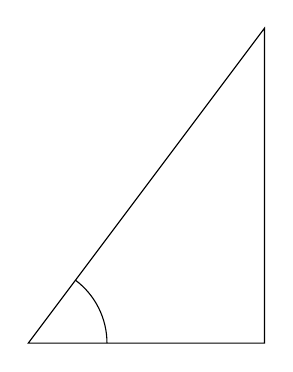
\begin{tikzpicture}
	%\draw (0,0) -- (10,0);
	%\draw (0,0) -- (0,10);
	%\draw (4,0) circle [radius=1];
	%\draw (3,5) rectangle (5,8);
	%\draw (4,0) arc [start angle = 0,end angle = 45,radius=4];
	\draw (3,0) -- (6,0) -- (6,4) -- cycle;
	\draw (4,0) arc [start angle = 0, end angle = 53, radius = 1];
\end{tikzpicture}
\end{document}
